\section{Tracks}
\label{sec:tracks}

\subsection{Track reconstruction}

To cite: \cite{soft-pub-2007-007}

\textbf{Inside out:}
\begin{itemize}
	\item Cluster formation
	\item Seed finding: reco triplets of hits from the pixel detector
	\item Track fitting with a combinatorial Kalman filter
	\item Ambiguity solving of which hits with a collection of NNs which decides whether a given cluster is shared between two tracks and how to split the energy depostion between these multiple tracks \cite{jinst-9-2014-P09009}
	\item Extend to the TRT hits
\end{itemize}

Improve the efficiency due to tracks in that have decays displaced from the original collision point with an \textbf{outside in:} track reconstruction alrogihm
\begin{itemize}
	\item Start with the seeds from the TRT
	\item Extend to the hits in the silicon detector
	\item Again use an ambiguity solver.
\end{itemize}

\begin{figure}[hbt]
\centering
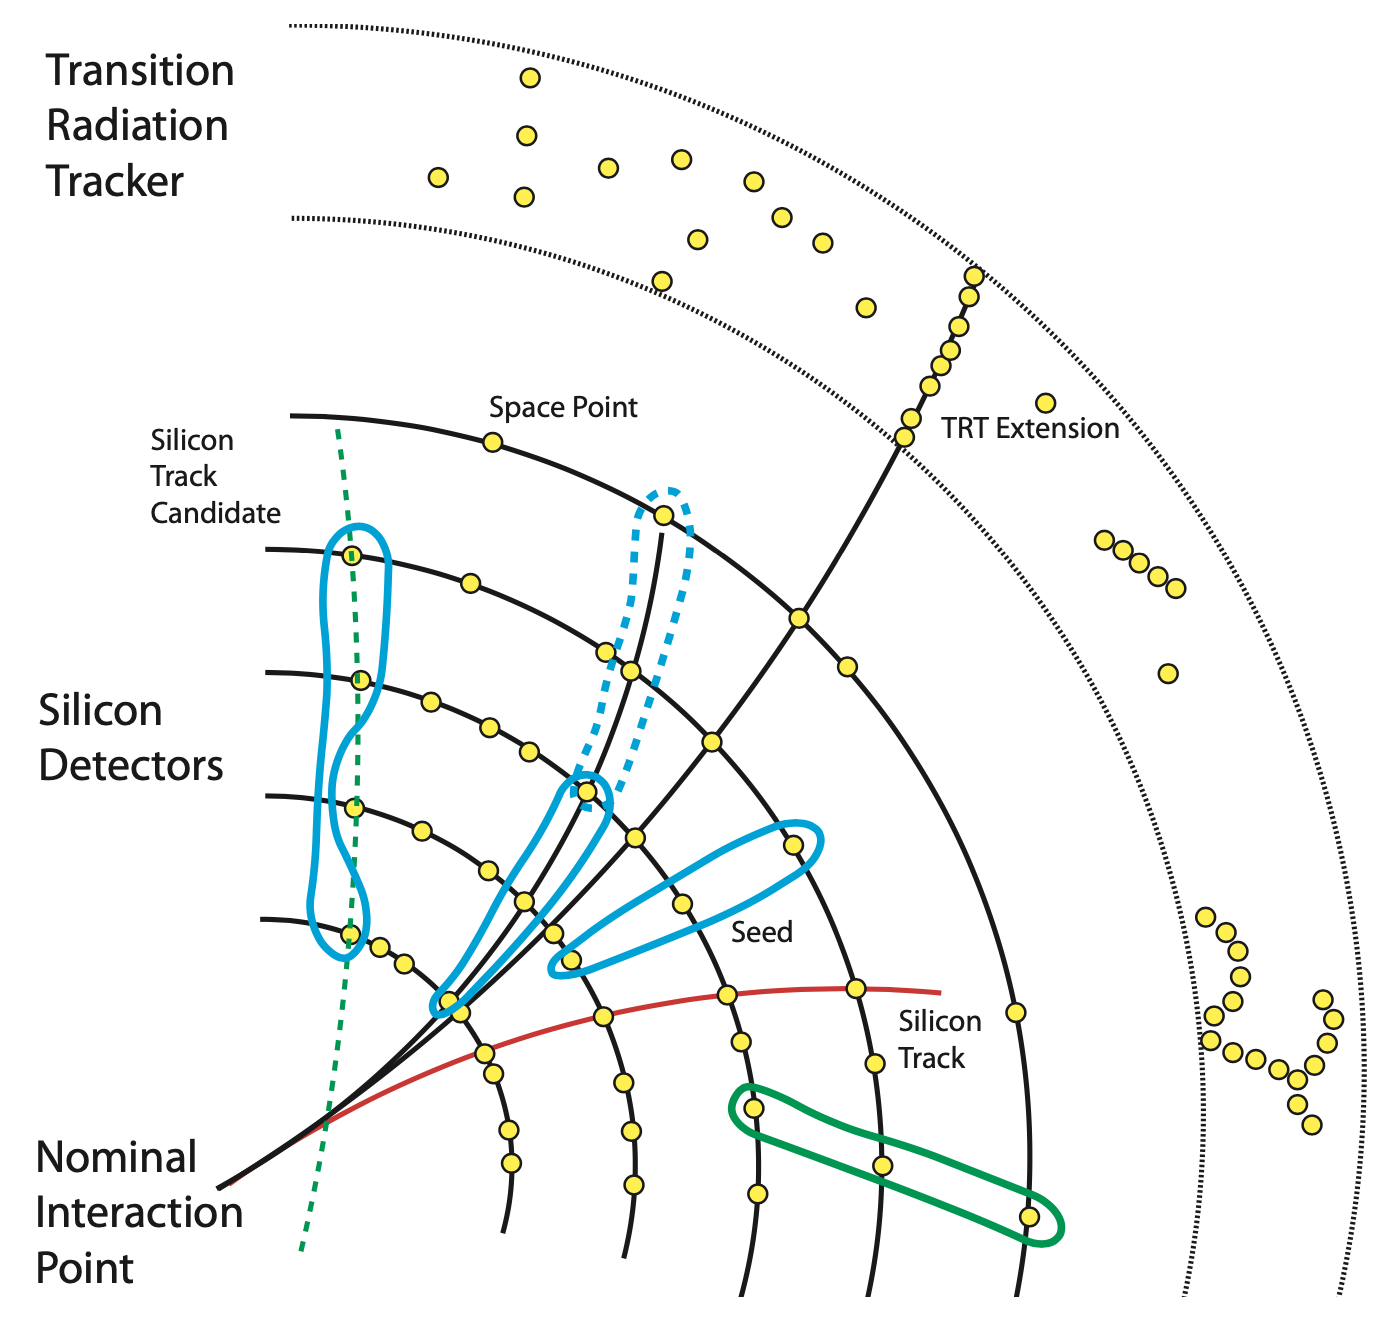
\includegraphics[width=0.6\textwidth]{figures/cp-graphics/tracking/track-reco}
\caption{\hl{need to ask Valentina where this pic was from originally}.}
\label{fig:track-reco}
\end{figure}


\subsection{Challenges in Dense Environments}

\begin{figure}[hbt]
\centering
\subfloat[]{
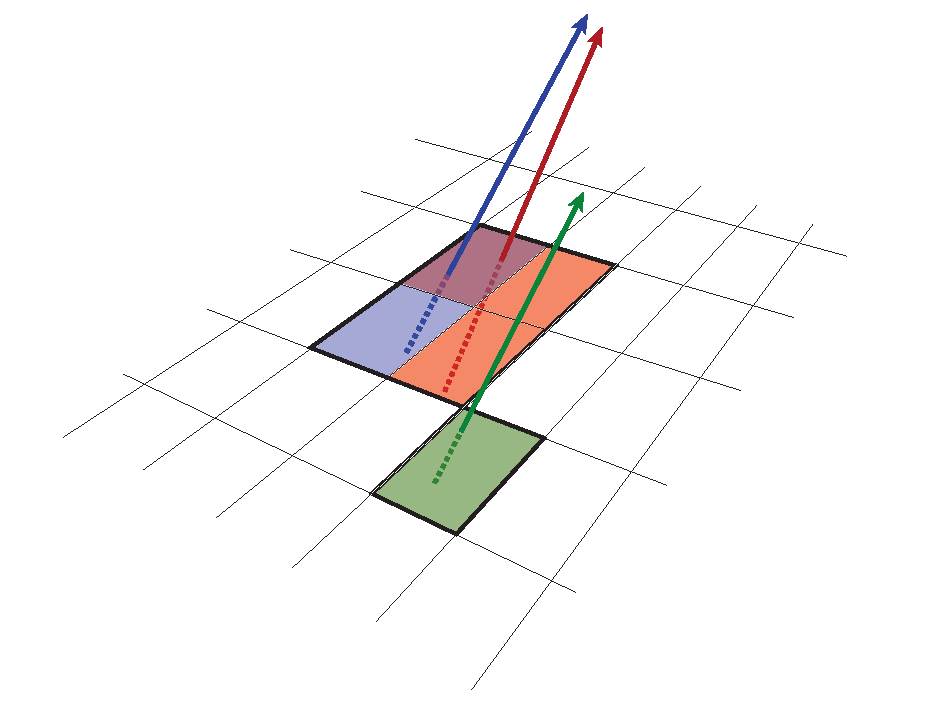
\includegraphics[width=0.43\textwidth]{figures/cp-graphics/jinst-9-2014-P09009/fig_03}
}
\subfloat[]{
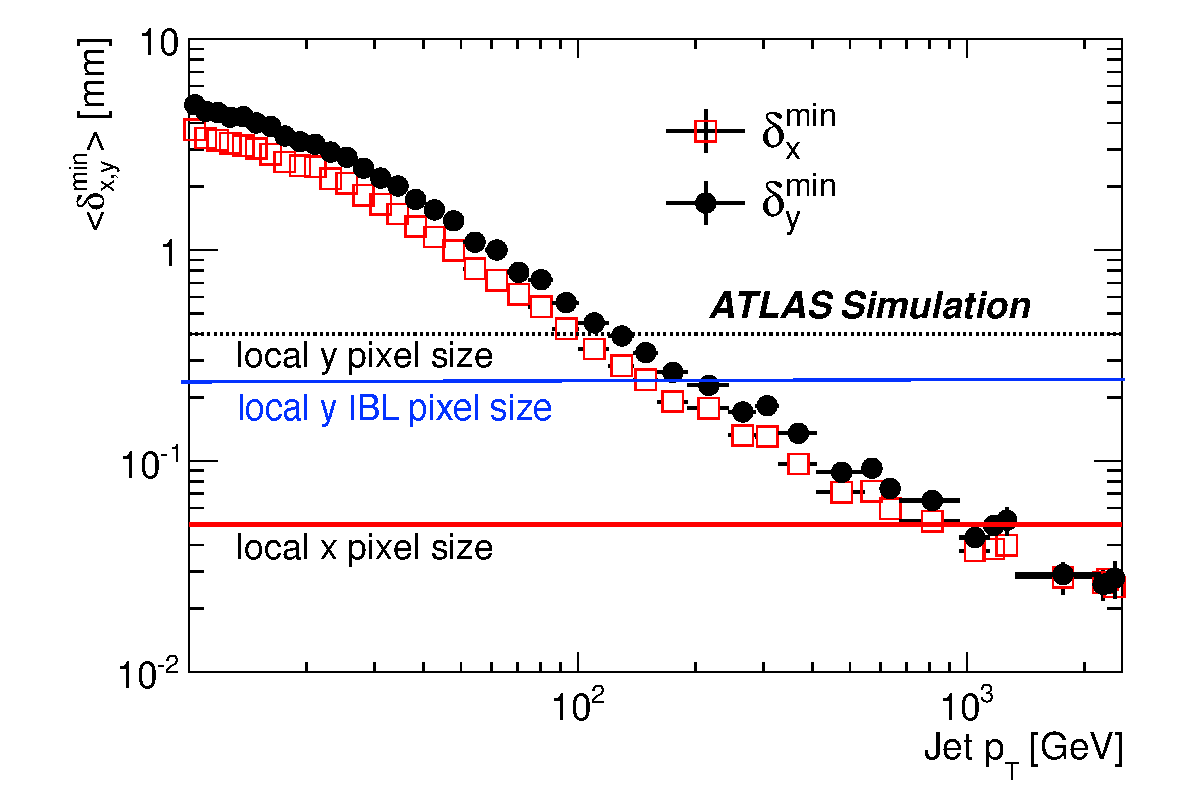
\includegraphics[width=0.55\textwidth]{figures/cp-graphics/jinst-9-2014-P09009/fig_04}
}
\caption{\cite{jinst-9-2014-P09009}.}
\label{fig:ctide}
\end{figure}


\subsection{Discussion of inputs}


\begin{figure}[hbt]
\centering
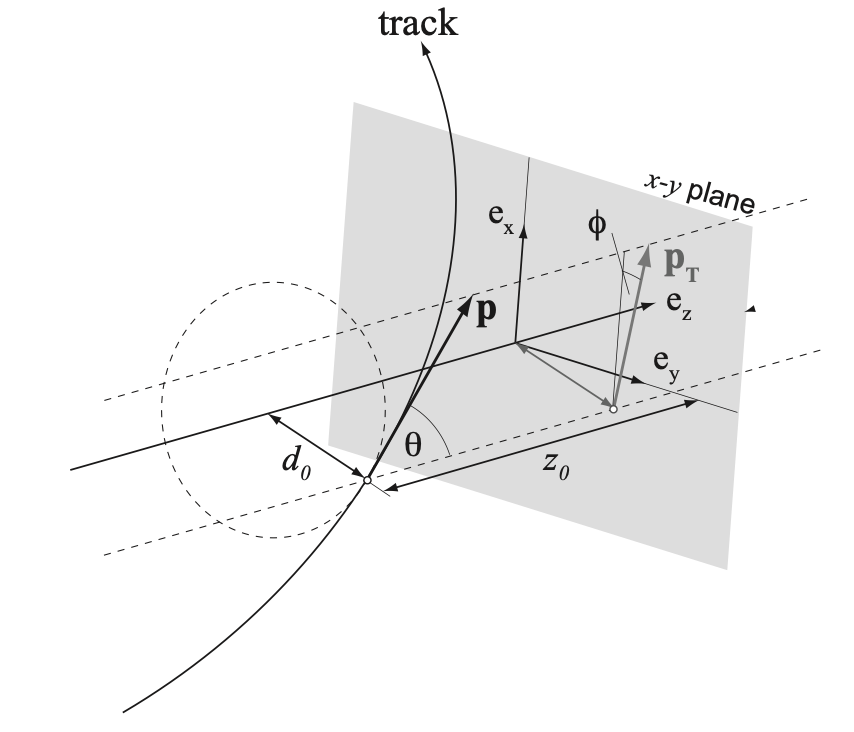
\includegraphics[width=0.6\textwidth]{figures/cp-graphics/ATL-SOFT-PUB-2007-003/fig-2a}
\caption{\cite{ATL-SOFT-PUB-2007-003}}
\label{fig:ATL-SOFT-PUB-2007-003-fig-2a}
\end{figure}

\begin{figure}[hbt]
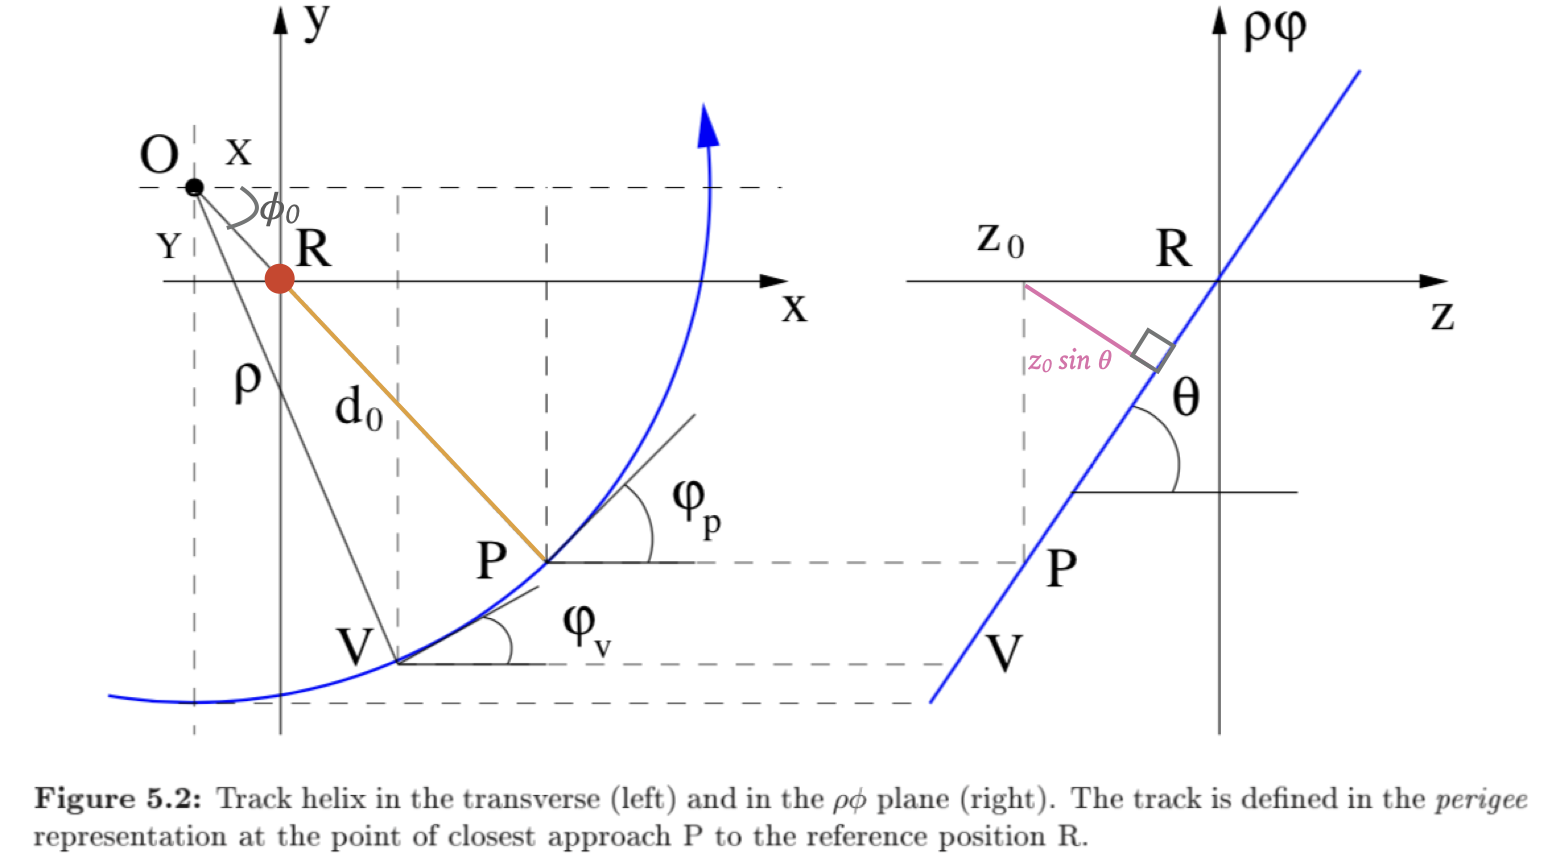
\includegraphics[width=\textwidth]{figures/cp-graphics/giacinto-fig-5.2}
\caption{\cite{giacinto-thesis}}
\label{fig:track-2d-graphics}
\end{figure}

\begin{itemize}
	\item \textcolor{red}{R}: reference position at which the tracks are defined, i.e, for \Pqb-tagging we use the primary vertex of the collision as the reference point. 
	\item \textcolor{orange}{$d_0$}:  The transverse impact parameter, point of closest approach (POCA) in the transverse plane with respect to R.
	\item \textcolor{pink}{$z_0 \sin \theta$}:  The longitudinal impact parameter, or the longitudinal displacement from the POCA (defined in the transverse plane). The multiplication by $\sin \theta$ term is included because it characterizes the 2d distance from $z_0$ to the closest point along the track trajectory.
\end{itemize}


\begin{align}
x_V &= x_R + d_0 \cos \left( \phi_p + \frac{\pi}{2} \right)+ \rho \left[  \cos \left( \phi_V + \frac{\pi}{2}  -  \cos \left( \phi_p + \frac{\pi}{2} \right)\right)  \right] \notag \\
y_V &= y_R + d_0 \sin \left( \phi_p + \frac{\pi}{2} \right)+ \rho \left[  \sin \left( \phi_V + \frac{\pi}{2}  -  \sin \left( \phi_p + \frac{\pi}{2} \right)\right)  \right] \\
z_V &= z_R + z_0 - \frac{\rho}{\tan \left( \theta \right) } \left[ \phi_V - \phi_p \right] \notag
\end{align}

\begin{figure}[hbt]
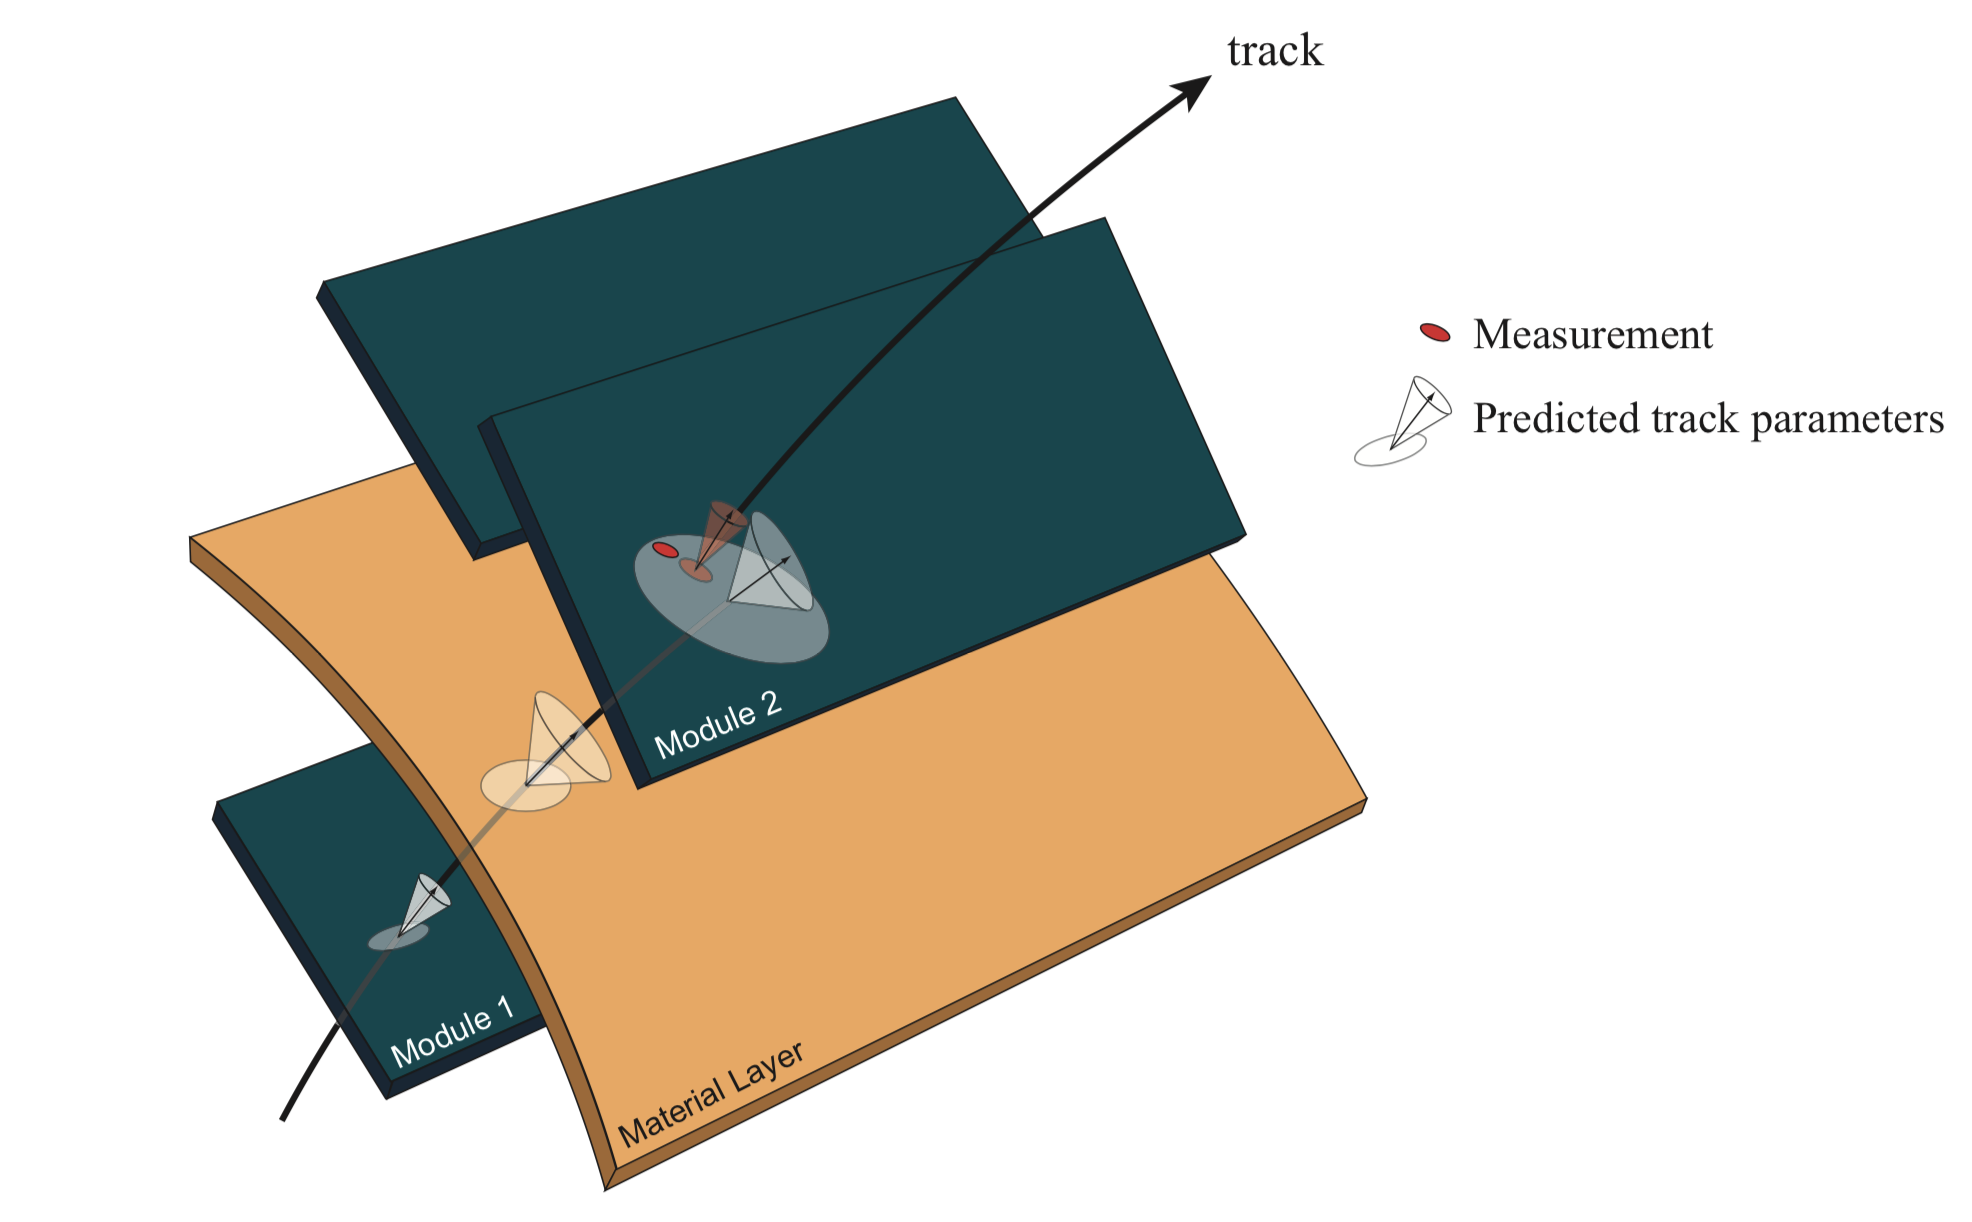
\includegraphics[width=\textwidth]{figures/cp-graphics/ATL-SOFT-PUB-2007-005/track-extrap-material-int}
\caption{Visualization of the track extrapolation with its associated errors \cite{ATL-SOFT-PUB-2007-005}.}
\label{fig:track-extrap-material-int}
\end{figure}

\begin{equation}
\rho = \frac{\sin \theta}{\frac{q}{p} B_z}
\end{equation}

\begin{align}
d_0 &= \text{sign} \left( d_0 - \rho \right) \sqrt{\left(x_V - x_R - \rho \cos \left(\phi_V + \frac{\pi}{2} \right) \right)^2 +  \left(y_V - y_R - \rho \sin \left(\phi_V + \frac{\pi}{2} \right) \right)^2 } \\
\phi_p &= \arctan \left( \frac{y_V - y_R - \rho \sin \left( \phi_V + \frac{\pi}{2}\right)}{x_V - x_R - \rho \cos \left( \phi_V + \frac{\pi}{2}\right)} \right) \\
z_0 &= z_R + z_V + \frac{\rho}{\tan \theta } \left[ \phi_V - \phi_p (x_V, y_V, z_V, \theta, q/p) \right]\\
\left( \frac{q}{p} \right)_P &= \left( \frac{q}{p} \right)_V \\
\theta_P &= \theta_V
\end{align}

The way we map from one representation to another is by calculating the Jacobians of the transformations:

\begin{equation}
A = \frac{\partial (d_0, z_0, \phi_P, \theta_P, q/p)}{\partial (x_V, y_V, z_V)} = 
\begin{bmatrix}
- h \frac{X}{S} & - h \frac{Y}{S} & 0 \\
\frac{\rho}{\tan \theta}  \frac{Y}{S^2} & - \frac{\rho}{\tan \theta}  \frac{X}{S^2}  & 1 \\
- \frac{Y}{S^2} &  \frac{X}{S^2} & 0 \\
0 & 0 & 0 \\
0 & 0 & 0
\end{bmatrix}
\end{equation}

\begin{equation}
B =  \frac{\partial (d_0, z_0, \phi_P, \theta_P, q/p)}{\partial (\phi_V, \theta, q/p)} = 
\begin{bmatrix}
- \frac{h \rho}{S} R & \frac{\rho}{\tan \theta} \left[ 1 - \frac{h}{S} R \right]  & - \frac{\rho}{q/p} \left[ \Delta \phi - \frac{h}{S} R  \right]  \\
\frac{\rho}{\tan \theta}  \left[ 1 - \frac{\rho}{S^2} Q \right] & \rho \left[ \Delta \phi + \frac{\rho}{S^2 \tan^2 \theta } R \right] & \frac{\rho}{q/p \tan \theta}\left[ \Delta \phi - \frac{\rho}{S^2} R \right] \\
\frac{\rho}{S^2} Q & - \frac{\rho}{S^2 \tan \theta}   R & \frac{\rho}{S^2 q/p}   R \\
0 & 1 & 0 \\
0 & 0 & 1 
\end{bmatrix}
\end{equation}


where:
\begin{align*}
X &= x_V - x_R - \rho \cos \left(\phi_V + \frac{\pi}{2} \right) 
Y &= y_V - y_R - \rho \sin \left( \phi_V + \frac{\pi}{2}\right)
R &= Y \sin \phi_V + X \cos \phi_V \\
Q &= X \sin \phi_V - Y \cos \phi_V \\
S &= \sqrt{X^2 + Y^2} \\
h &= \text{sign}  \rho \\
\phi &= \phi_P - \phi_V
\end{align*}

\textbf{Q:} How do we define the sign of $\rho$?

\subsection{The perigee parameters}